\documentclass{article}

\usepackage{graphicx}
\usepackage{tikz}
\usepackage{tikzsymbols}
\usetikzlibrary{calc,patterns,shapes.geometric}
\pagestyle{empty}
\usepackage[margin=0pt]{geometry}
\geometry{papersize={14in,12in}}

\def\centerarc[#1](#2)(#3:#4:#5){\draw[#1] ($(#2)+({#5*cos(#3)},{#5*sin(#3)})$) arc (#3:#4:#5);}

\begin{document}
	\begin{figure}
		\centering
		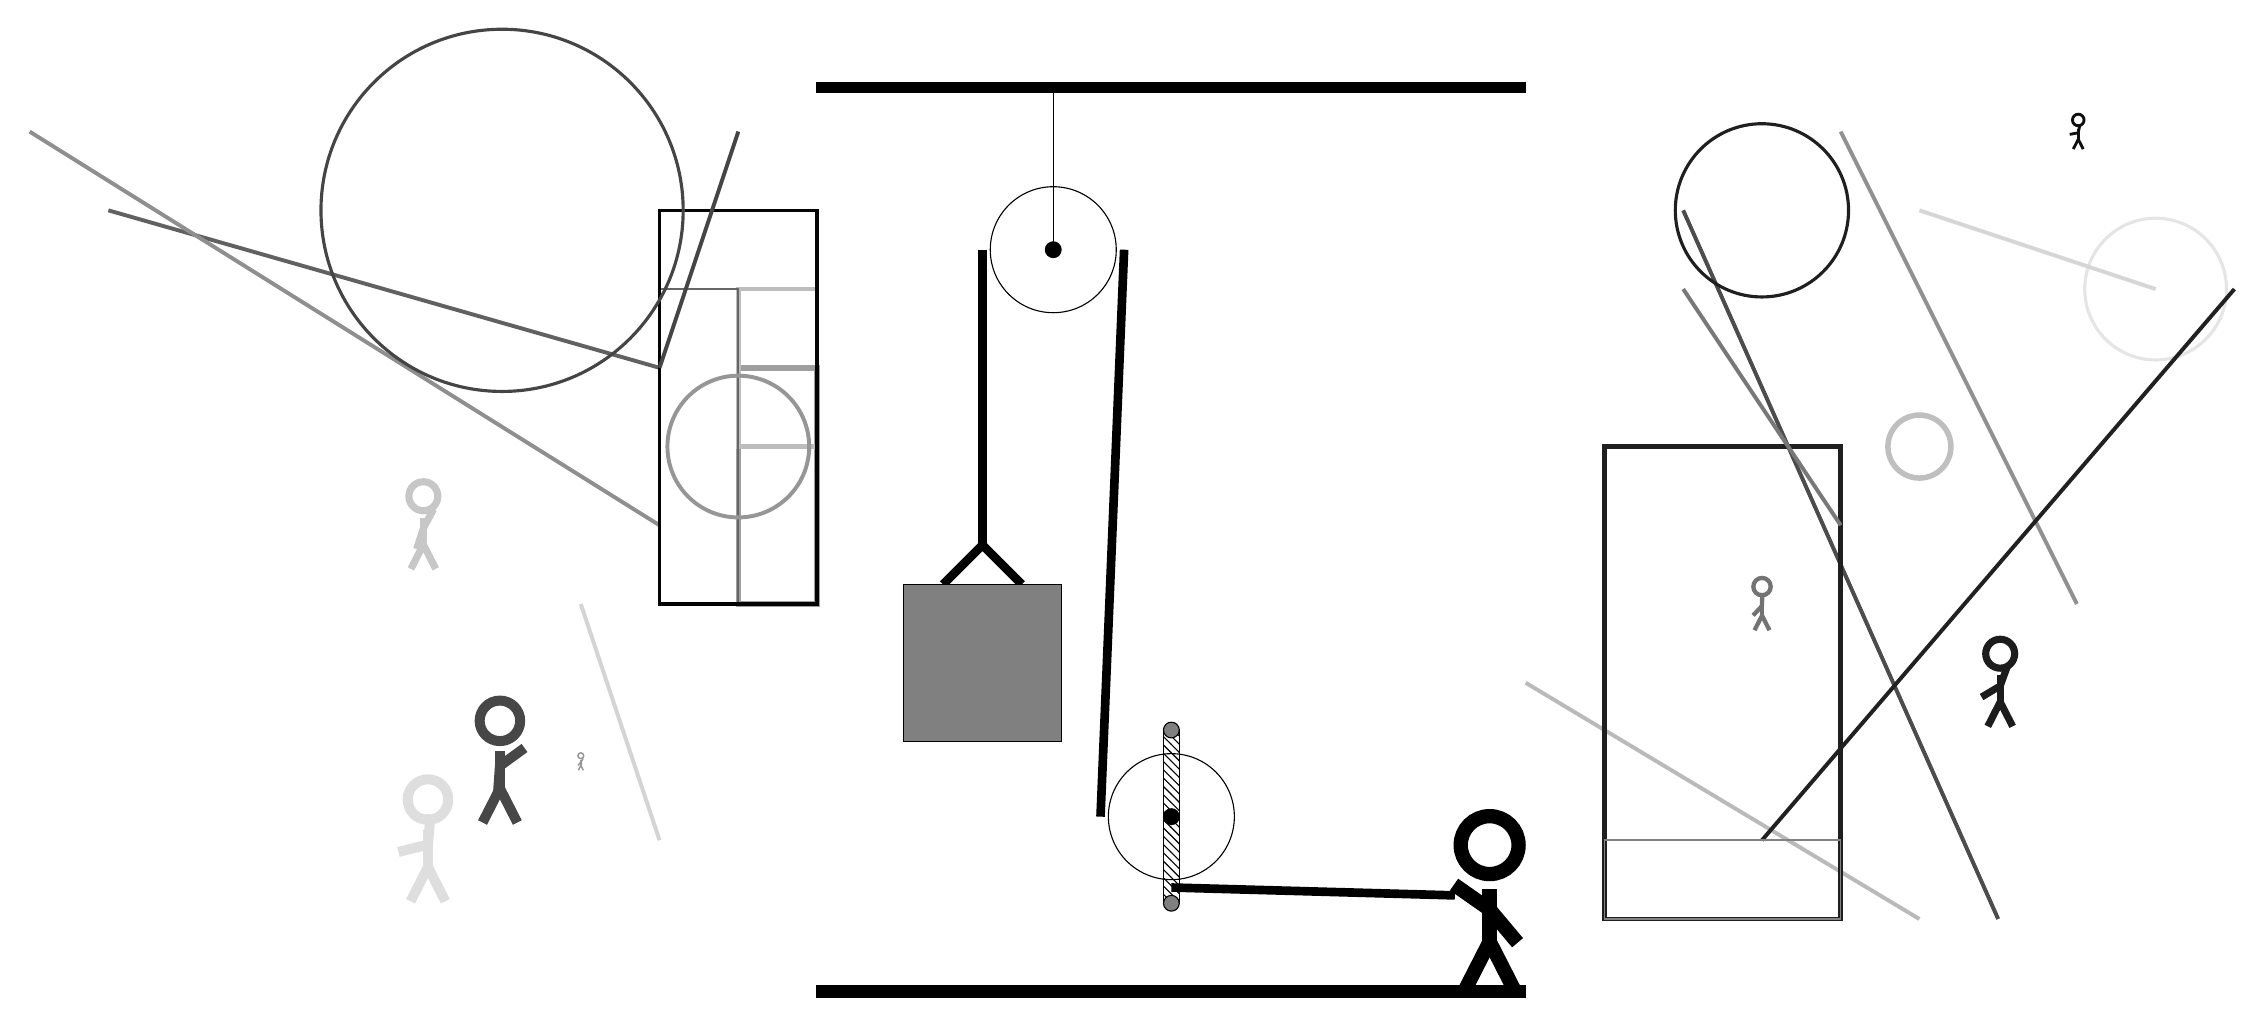
\begin{tikzpicture}
			%%%%% START %%%%%
			
			\draw[fill=black] (-2, 11.5) rectangle (7, 11.625);
			
			\draw (1, 9.5) circle (0.8);
			\draw[fill=black] (1, 9.5) circle (0.1);
			\draw (1, 11.5) -- (1, 9.5);
			
			\draw[fill=white](2.5, 2.3) circle (0.8);
			\draw[fill=black] (2.5, 2.3) circle (0.1);
			\draw[pattern=north west lines, pattern color=black] (2.4, 3.4) rectangle (2.6, 1.2);
			\draw[fill=black!50] (2.5, 3.4) circle (0.1);
			\draw[fill=black!50] (2.5, 1.2) circle (0.1);
			
			\draw[line width=1.1mm] (-0.4, 5.25) -- (0.1, 5.75) -- (0.6, 5.25);
			\draw[fill=black!50] (-0.9, 5.25) rectangle (1.1, 3.25);
			
			\draw[line width=1.1mm] (0.1, 9.5) -- (0.1, 5.75);
			\centerarc[line width=1.1mm](1, 9.5)(0:180:0.9);
			\draw[line width=1.1mm](1.9, 9.5) -- (1.6, 2.3);
			\centerarc[line width=1.1mm](2.5, 2.3)(180:270:0.9);
			\draw[line width=1.1mm](2.5, 1.4) -- (6.1, 1.3);
			
			\node at (6.5, 1.2) {\Strichmaxerl[10][-35][-50]};
			
			\node[line width=0.2mm, color=black!94] at (14, 11) {\Strichmaxerl[2][10][79]};
			
			\draw[line width=0.5mm, color=black!62](-4, 8) -- (-11, 10);
			\draw[line width=0.7mm, color=black!38] (-2, 8) rectangle (-3, 5);
			\draw[line width=0.6mm, color=black!26] (-2, 9) rectangle (-3, 7);
			\draw[line width=0.5mm, color=black!17](-4, 2) -- (-5, 5);
			
			\draw[line width=0.5mm, color=black!44](-4, 6) -- (-12, 11);
			\draw[line width=0.3mm, color=black!60] (-3, 5) rectangle (-4, 9);
			\node[line width=0.6mm, color=black!42] at (-5, 3) {\Strichmaxerl[1][48][57]};
			\draw[line width=0.5mm, color=black!43](11, 11) -- (14, 5);
			\draw[line width=0.5mm, color=black!27](12, 1) -- (7, 4);
			\draw[line width=0.4mm, color=black!98] (-4, 5) rectangle (-2, 10);
			\node[line width=0.7mm, color=black!22] at (-7, 6) {\Strichmaxerl[5][72][62]};
			\draw [line width=0.4mm, color=black!10](15, 9) circle (0.9);
			\draw[line width=0.5mm, color=black!70](9, 10) -- (13, 1);
			\draw [line width=0.7mm, color=black!25](12, 7) circle (0.4);
			\draw [line width=0.2mm, color=black!69](-8, 6) circle (0.0);
			
			\node[line width=0.3mm, color=black!55] at (10, 5) {\Strichmaxerl[3][47][89]};
			\draw [line width=0.5mm, color=black!41](-3, 7) circle (0.9);
			\draw[line width=0.6mm, color=black!88] (8, 7) rectangle (11, 1);
			\draw[line width=0.5mm, color=black!16](12, 10) -- (15, 9);
			\draw[line width=0.5mm, color=black!87](10, 2) -- (16, 9);
			
			\node[line width=0.3mm, color=black!72] at (-6, 3) {\Strichmaxerl[7][86][36]};
			\node[line width=0.7mm, color=black!13] at (-7, 2) {\Strichmaxerl[7][14][85]};
			\draw [line width=0.4mm, color=black!88](10, 10) circle (1.1);
			\draw[line width=0.5mm, color=black!53](9, 9) -- (11, 6);
			\node[line width=0.7mm, color=black!89] at (13, 4) {\Strichmaxerl[5][31][70]};
			
			\draw[line width=0.2mm, color=black!49] (8, 2) rectangle (11, 1);
			\draw[line width=0.5mm, color=black!73](-3, 11) -- (-4, 8);
			\draw [line width=0.4mm, color=black!73](-6, 10) circle (2.3);
			
			\draw[fill=black] (-2, 0) rectangle (7, 0.15);
			
			%%%%% END %%%%%
		\end{tikzpicture}
	\end{figure}	
\end{document}